\let\negmedspace\undefined
\let\negthickspace\undefined
\documentclass[journal]{IEEEtran}
\usepackage[a5paper, margin=10mm, onecolumn]{geometry}
\usepackage{tfrupee} 

\setlength{\headheight}{1cm}
\setlength{\headsep}{0mm}

\usepackage{gvv-book}
\usepackage{gvv}
\usepackage{cite}
\usepackage{amsmath,amssymb,amsfonts,amsthm}
\usepackage{algorithmic}
\usepackage{graphicx}
\usepackage{textcomp}
\usepackage{xcolor}
\usepackage{txfonts}
\usepackage{listings}
\usepackage{enumitem}
\usepackage{mathtools}
\usepackage{gensymb}
\usepackage{comment}
\usepackage[breaklinks=true]{hyperref}
\usepackage{tkz-euclide} 
\usepackage{listings}

\def\inputGnumericTable{}                                 
\usepackage[latin1]{inputenc}                                
\usepackage{color}                                            
\usepackage{array}                                            
\usepackage{longtable}                                       
\usepackage{calc}                                             
\usepackage{multirow}                                         
\usepackage{hhline}                                           
\usepackage{ifthen}                                           
\usepackage{lscape}

\title{\textbf{4.2.9}}
\author{\textbf{EE25BTECH11006 - ADUDOTLA SRIVIDYA}}
\date{september 11, 2025}

\begin{document}

\maketitle

\section*{\textbf{Question}}
Find the direction vector and the normal vector of the line $x + y = 4$.

\section*{\textbf{Solution}}

The line can be written as: 
\begin{align}
x + y = 2
\end{align}

This equation can be expressed in terms of matrices\\
Let
\begin{align}
\vec{x} = \myvec{x \\ y}
\end{align}
\begin{align}
\vec{n^T} = \myvec{1 & 1}
\end{align}
\begin{align}
c = 4
\end{align}

The line equation can be written as:
\begin{align}
\vec{n^T}  \vec{x} = c
\end{align}

Where $\vec{n}$ is the normal vector of the given line

The direction vector of the line can be found by observing the normal vector.
\begin{align}
\vec{m} = \myvec{-1 \\ 1}
\end{align}



This is true because if the director vector is represented as 
\begin{align}
\vec{m}  = \myvec{1 \\ m}    
\end{align}
then the normal vector can be represented as 
\begin{align}
\vec{n} = \myvec{-m \\ 1}
\end{align}

This can be verified by the following equation:
\begin{align}
\vec{n^T}\vec{m} = 0
\end{align}

\begin{align}
\myvec{1 & 1}\myvec{-1 \\ 1} = 0
\end{align}\\



The normal vector of the line is $\vec{n} = \myvec{1 \\ 1}$
The director vector of the line is $\vec{m} = \myvec{-1 \\ 1}$\\

\begin{figure}[H]
    \centering
    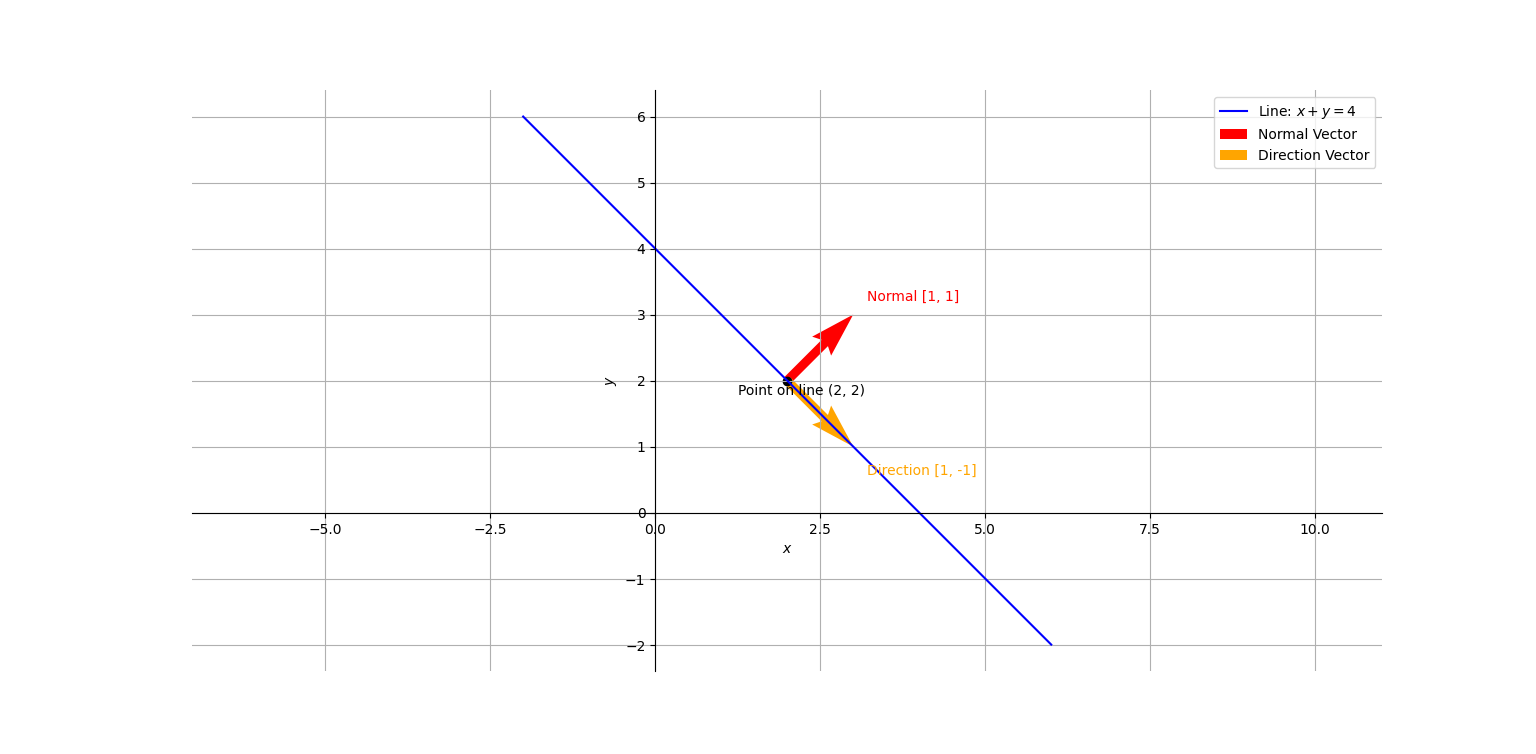
\includegraphics[width=1.1\columnwidth]{figs/fig6.png}
    \caption{Line $x + y = 4$ with its normal and direction vectors}
    \label{fig:placeholder}
\end{figure}

\end{document}